\documentclass[11pt]{article} % 
\usepackage[pdftex]{graphicx}
\usepackage{fullpage}
\usepackage{graphicx}
\usepackage{graphics}
\usepackage{psfrag}
\usepackage{pgf}
\usepackage{color}
\usepackage{tikz}
\usepackage{epstopdf}
\usetikzlibrary{arrows,automata}
\usepackage[latin1]{inputenc}
\usepackage{amsthm}
\usepackage{amsmath,amssymb}
\usepackage{enumerate}
\setlength{\textwidth}{6.5in}
\setlength{\textheight}{9in}
\newcommand{\N}{\mathbb{N}}
\newcommand{\Z}{\mathbb{Z}}
\newcommand{\R}{\mathbb{R}}
\newcommand{\Q}{\mathbb{Q}}
\newcommand{\C}{\mathbb{C}}
\newcommand{\PP}{\mathbb{P}}
\newcommand{\tab}{\;\;\;\;\;}
\newcommand{\inv}{^{-1}}
\newcommand{\tr}{\textrm}
\newcommand{\lc}{\sqcup}
\newcommand{\var}{\tr{Var}}
\newcommand{\cov}{\tr{Cov}}
\newcommand{\like}{\mathcal{L}}

\begin{document}

\hfill Robert Johns

\hfill April 3, 2014

\begin{center} {\Large CSCI 678: Statistical Analysis of Simulation Models}\\{\large Homework 10}\end{center}

\begin{enumerate}

%%%%%
%1
\item For the MA(2) process:
$$X_t = \beta_0 Z_t + \beta_1 Z_{t-1} + \beta_2 Z_{t-2}$$
we have
\begin{align*}E[X_t] &= E[\beta_0 Z_t + \beta_1 Z_{t-1} + \beta_2 Z_{t-2}]\\
& = \beta_0 E[Z_t] + \beta_1 E[Z_{t-1}] + \beta_2 E[Z_{t-2}] \\
&= 0\end{align*}
because the expected value of each noise term is 0.  Also, because the noise terms are iid, we have that
\begin{align*}V[X_t] &= V[\beta_0 Z_t + \beta_1 Z_{t-1} + \beta_2 Z_{t-2}]\\
& = \beta_0^2 V[Z_t] + \beta_1^2 V[Z_{t-1}] + \beta_2^2 V[Z_{t-2}]\\
& = (\beta_0^2+\beta_1^2+\beta_2^2)\sigma_Z^2\end{align*}

Since $E[X_t] = E[X_{t+1}] =0$ we see that
$$\cov(X_t, X_{t+1}) = E[(\beta_0 Z_t + \beta_1 Z_{t-1} + \beta_2 Z_{t-2})(\beta_0 Z_{t+1} + \beta_1 Z_t + \beta_2 Z_{t-1})]$$
Because $E[Z_s Z_t]$ is $\sigma_Z^2$ if $s=t$ and $0$ otherwise, we see that
$$\gamma(1) = \beta_0\beta_1\sigma_Z^2 + \beta_1\beta_2\sigma_Z^2 = \beta_1(\beta_0+\beta_2)\sigma_Z^2$$
Similarly, for $\gamma(2)$, we have
$$\cov(X_t,X_{t+2}) = E[(\beta_0 Z_t + \beta_1 Z_{t-1} + \beta_2 Z_{t-2})(\beta_0 Z_{t+2} + \beta_1 Z_{t+1} + \beta_2 Z_t)] = \beta_0\beta_2\sigma_Z^2$$
A pattern emerges: we see see that $\gamma(k) = 0$ for $|k|>2$, so the autocorrelation function for an MA(2) process is
$$\rho(k) =\begin{cases}
1 &  k = 0 \\
\frac{\beta_1(\beta_0+\beta_2)}{\beta_0^2+\beta_1^2+\beta_2^2}       & k = 1, -1\\
\frac{\beta_0\beta_2}{\beta_0^2+\beta_1^2+\beta_2^2} &k = 2, -2\\
0 & |k| > 2
\end{cases}$$

%%%%%
%2
\item

\begin{enumerate}

%2a
\item We can alternately express this model as $X_t = \Theta(B)Z_t$, where $\Theta(B) = 1 + 2B+10B^2$ and $B$ is the backshift operator.  From the notes, we know that the model is invertible if the roots of $\Theta(B)$ lie outside the complex unit circle. Applying the quadratic formula, we see that the roots of $\Theta(B)$ are $-1+ 6i$ and $-1 - 6i$, so the model in invertible.

%2b
\item $\\$
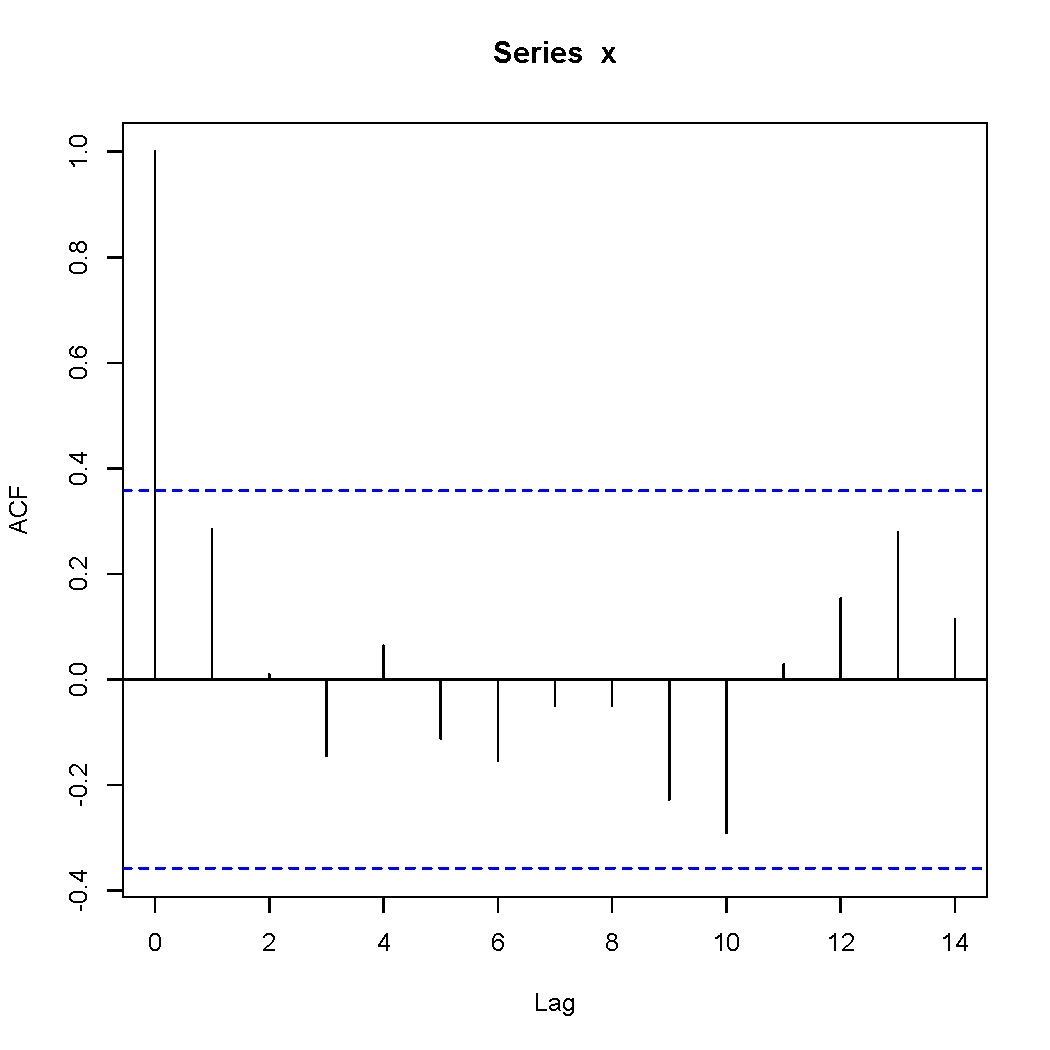
\includegraphics[scale = .35]{plot3.pdf}

%2c
\item The program \texttt{asm10a.r} was used to create the function. The code and plot of the results are below:

\begin{verbatim}realma <- function(iq, parms, xmu, sig, n) {
realma <- function(iq, parms, xmu, sig, n) {
       x = c(1:n)
       z = rnorm(iq, xmu, sig)
       T = c(1:n)
       t = 0
       while (t < n) {
       	     t = t + 1
	     z = c(rnorm(1,xmu,sig), z)
	     for (i in 1:iq){
	     	 x[t] = parms[i]*z[i]}
	}
	plot(T,x, type = "l")
	return(x)
}\end{verbatim}

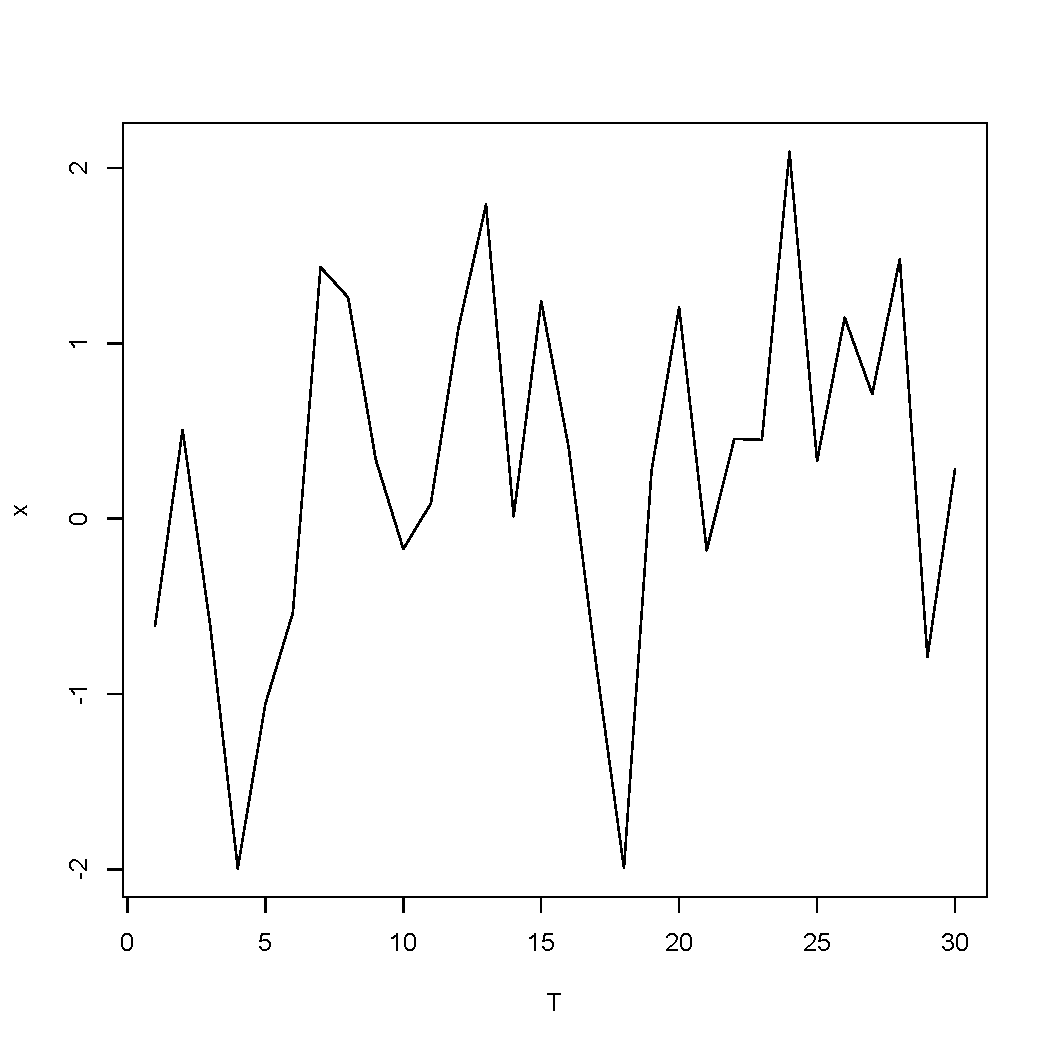
\includegraphics[scale = .4]{plot4.pdf}

\end{enumerate}

%%%%%
%3
\item

\begin{enumerate}

%3a
\item Using a backshift operator, we can express this model as $X_t = \Theta(B)Z_t$, where $\Theta(B) = 3 - 2B$ and $B$ is the backshift operator. From the notes, we know that the model will be invertible if $|-\frac{3}{2}|>1$.  Since $|-\frac{3}{2}| = \frac{3}{2} > 1$, we see that the model is invertible.

%3b
\item $\\$
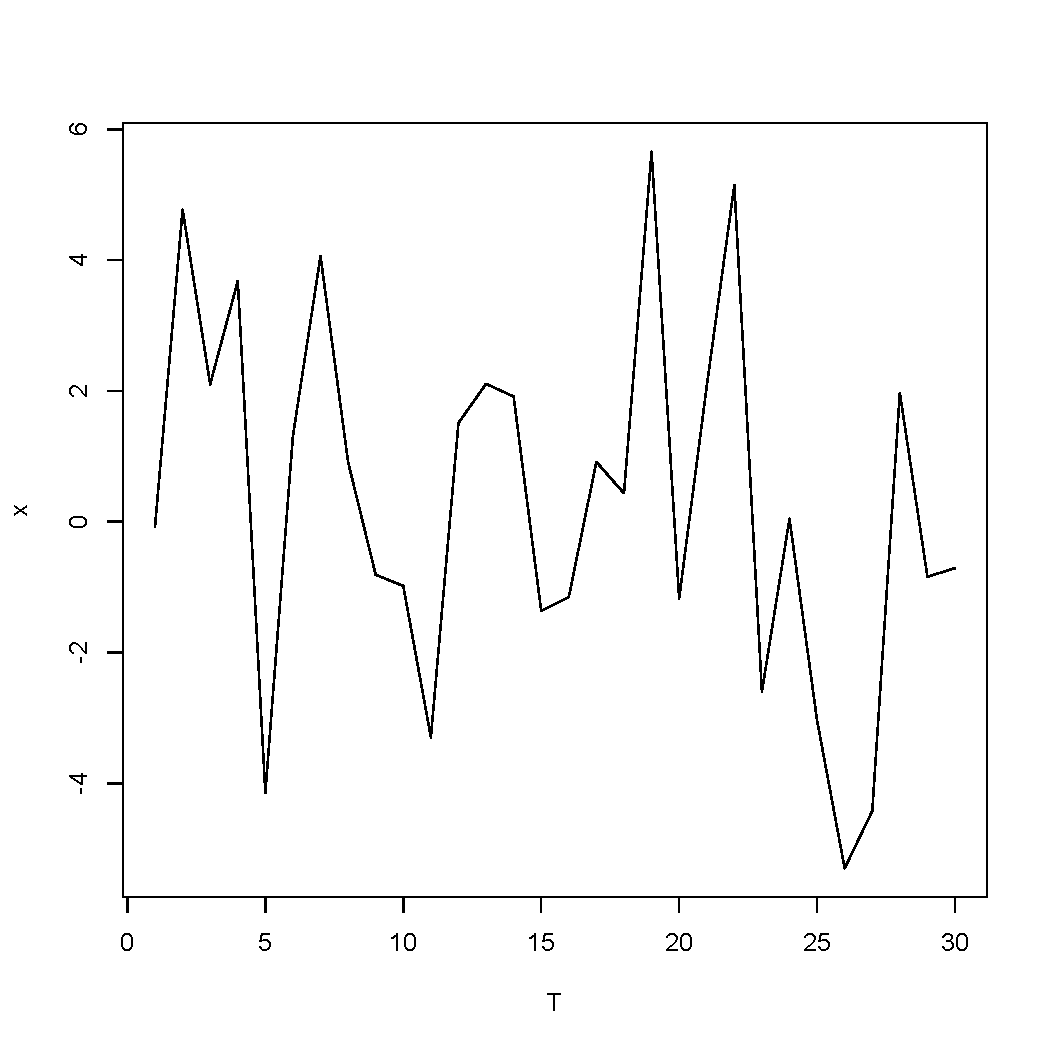
\includegraphics[scale = .4]{plot5.pdf}

%3c
\item The same program \texttt{asm10a.r} was used to produce the following plot:

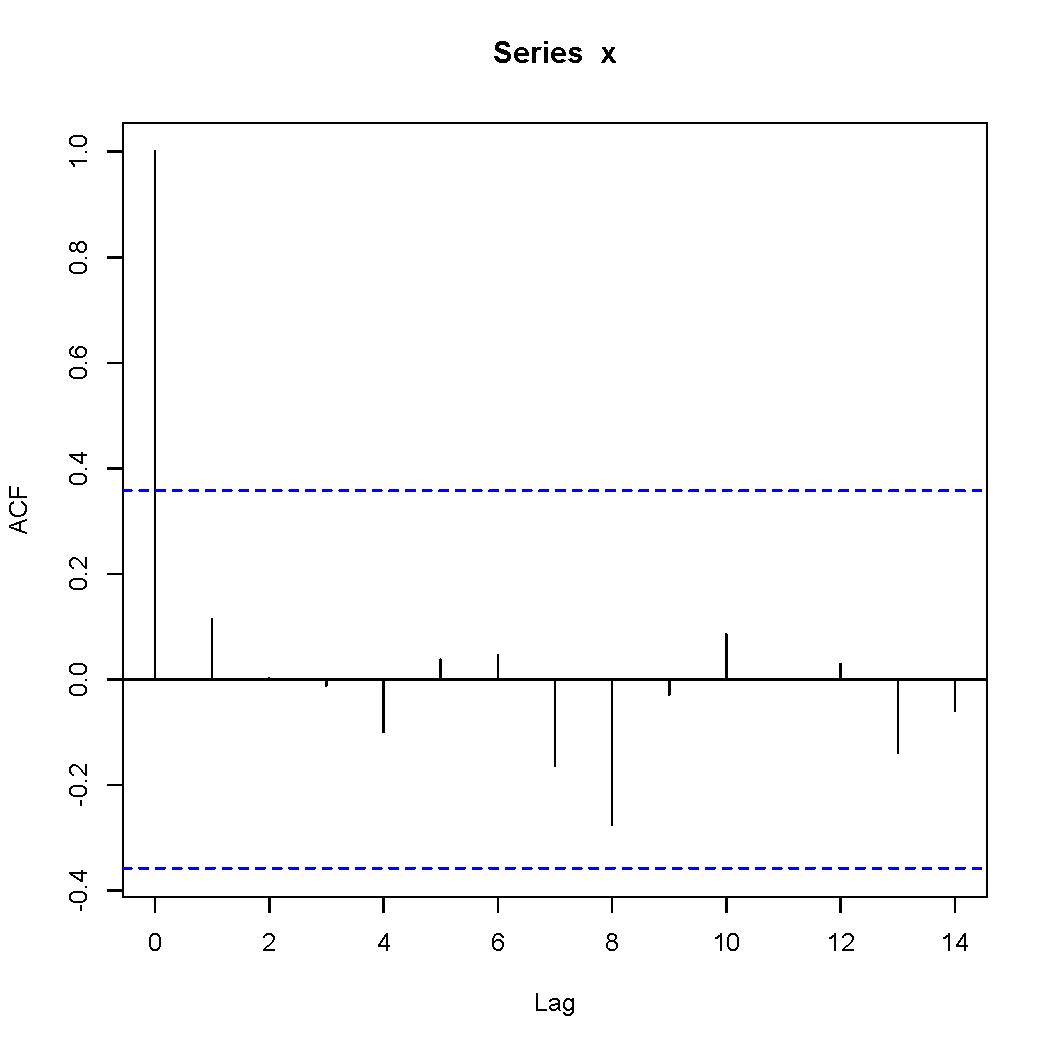
\includegraphics[scale = .4]{plot6.pdf}

\end{enumerate}

%%%%%
%4
\item Applying the result from question 1, we have that
\begin{align*}\rho(0) &= 1\\
\rho(1) &= \frac{\beta_1(\beta_0+\beta_2)}{\beta_0^2+\beta_1^2+\beta_2^2} = \frac{0.7(1-0.2)}{1+0.49+0.04} = 0.366013\\
\rho(2) &= \frac{\beta_0\beta_2}{\beta_0^2+\beta_1^2+\beta_2^2} = \frac{-0.2}{1+0.49+0.04} = -0.13071895\end{align*}

As the model is MA(2), the $\rho(k) = 0$ for all $k > 2$.

\newpage

%%%%%
%5
\item The model under consideration is $X_t = \sum_{k=0}^m \frac{Z_{t-k}}{m+1}$. Because the expected value of the noise terms is 0, we see that $E[X_t] = 0, V[X_t] = \sigma_Z^2$. So then:
\begin{align*}\cov(X_t, X_{t+k}) &= E\left[\left(\frac{Z_t}{m+1}+\frac{Z_{t-1}}{m+1}+\ldots+\frac{Z_{t-m}}{m+1}\right)\left(\frac{Z_{t+k}}{m+1}+\frac{Z_{t+k-1}}{m+1}+\ldots+\frac{Z_{t+k-m}}{m+1}\right)\right]\\
&= \frac{1}{m+1}E[(Z+t + Z_{t-1} + \ldots + Z_{t-m})(Z_{t+k} + Z_{t+k-1} + \ldots + Z_{t+k-m})]\end{align*}
Because $E[Z_xZ_y] = 0$, all but $m+1-k$ terms will be 0, so $\cov(X_t, X_{t+k}) = \frac{m+1-k}{m+1}\sigma_Z^2$. So our acf is:
$$\rho(k)=
\begin{cases}
   1 &  k = 0 \\
    \frac{m+1-k}{m+1}    &  k = 1,\ldots,m\\
   0 &  k > m
  \end{cases}$$

%%%%%
%6
\item We see that the variance of the infinite order MA process $X_t = Z_t + C(Z_{t-1}+Z_{t-1}+\ldots)$ is:
\begin{align*}V[X_t] &= V[Z_t + C(Z_{t-1}+Z_{t-1}+\ldots)]\\
& = V[Z_t] + C^2(V[Z_{t-1}] + V[Z_{t-1}] + \ldots)\\
& = \sigma_Z^2 + C^2 \sum_{i=1}^\infty \sigma_Z^2\end{align*}
So, as the variance is infinite, the process is non-stationary.
  
For the series of differences $Y_t = X_t-X_{t-1} = (Z_t + c\sum_{i=1}^\infty Z_{t-i}) - (Z_{t-1} + c\sum_{i=2}^{\infty}Z_{t-i}) = Z_t +(C-1)Z_{t-1}$, we have that $E[Y_t] = 0$ and $V[Y_t] = (C^2-2C+2)\sigma_Z^2$, which are both constant, so the series is stationary. The autocorrelation function for $Y_t$ is:
$$\rho(k)= \begin{cases}
1 &  k = 0 \\
\frac{C-1}{C^2-2C+2}    &  k = 1\\
0 &  k > 1
\end{cases}$$

%%%%%
%7
\item Our model is $X_t = \mu + Z_t + \beta Z_{t-1}$. We see that $E[X_t] = \mu$ and $V[X_t] = (1 + \beta^2)\sigma_Z^2$. We have that
$$\cov(X_t,X_{t+1}) = E[(X_t-\mu)*(X_{t+1}-\mu)] - E[X_t-\mu]*E[X_{t+1}-\mu]$$
Since the individual expectations are each 0, the covariance is the expectation of the product. Also
\begin{align*}E[(X_t-\mu)(X_{t+1}-\mu)] &= E[(\mu + Z_t + \beta Z_{t-1} - \mu)(\mu + Z_{t+1} + \beta Z_t-\mu)]\\
& = E[(Z_t + \beta Z_{t-1})(Z_{t+1} + \beta Z_t)]\end{align*}
which does not depend on $\mu$. The autocorrelation function is
$$\rho(k)=\begin{cases}
1 &  k = 0 \\
\frac{\beta}{1+\beta^2}    &  k = 1\\
0 &  k > 1
\end{cases}$$

%%%%%
%8
\item
\begin{enumerate}

%8a
\item In the following picture, $b1 = \beta_0, x = \beta_1$:

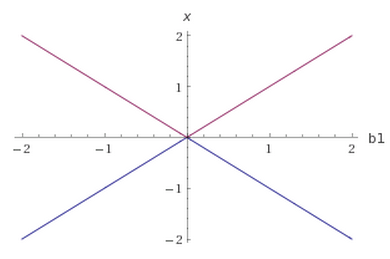
\includegraphics[scale=.6]{plot7.png}

%8b
\item On the edges of the invertibility region, $|\beta_0|=|\beta_1|=\beta$, so $\rho(1) = \frac{\beta_0 \beta_1}{\beta_0^2+\beta_1^2} = \pm \frac{\beta^2}{2\beta^2} = \pm \frac{1}{2}$. So we have that, $-0.5<\rho(1)<0.5$.

\end{enumerate}

%%%%%
%9
\item In the following picture (obtained from WolframAlpha), $l1 = \lambda_1, l2 = \lambda_2$

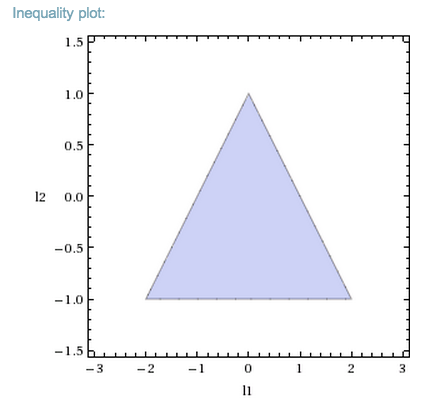
\includegraphics[scale = .4]{plot8.png}

The level curves are $\rho(1) = \frac{\lambda_1}{1 - \lambda_2} = .5$ and $\rho(2) = \frac{\lambda_1^2}{1 - \lambda_2} + \lambda_2$.

%%%%%
%10
\item We can rewrite the process as $(1-B-cB^2)X_t=Z_t$, where $B$ is the backshift operator. If the roots of $1-B-cB^2=0$ lie outside the unit circle, the process is stationary. From the quadratic formula, the roots are $\frac{1+ \sqrt{1+4c}}{2}$ and $\frac{1- \sqrt{1+4c}}{2}$. In polar form, radius is
$$r = \sqrt{\bigg(\frac{-1+ \sqrt{1+4c}}{2c}\bigg)\bigg(\frac{-1- \sqrt{1+4c}}{2c}\bigg)} = \sqrt{\frac{1-1-4c}{4c^2}} = \sqrt{\frac{-1}{c}}$$
So then to be invertible, we must have that $r > 1$, so $\sqrt{\frac{-1}{c}}>1$, which is true if $-1<c<0$.

Since $B=1$ is a root of the equation and lies on the unit circle, we see that the process is not stationary.

\newpage

%%%%%
%11
\item Two plots, one of the time series and one of the autocorrelation function, follow.

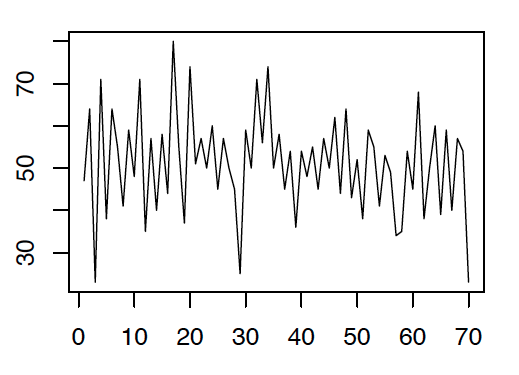
\includegraphics[scale=.5]{plot1.png}

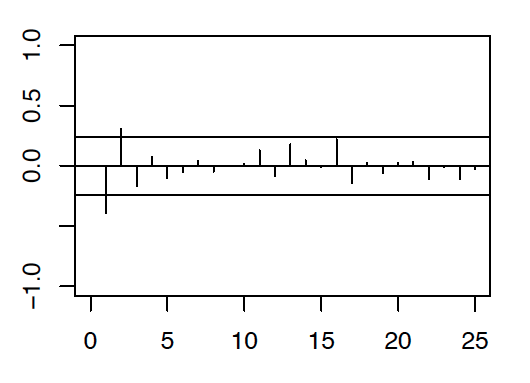
\includegraphics[scale = .5]{plot2.png}

\end{enumerate}

\end{document}

\end{document}